% data_sha256=e9d2a0731b838423e81f3b281eec33bf63364ddf6faebbcbce13969d5556a5cd
\pgfplotsset{briefaxis/.style={
font=\fontsize{9}{11}\selectfont, tick label style={text=black},
label style={text=black}, title style={text=black},
axis line style={black,line width=0.6pt}, tick style={black},
axis background/.style={fill=white}, grid style={black!12},
legend style={text=black,font=\fontsize{9}{11}\selectfont,draw=none,fill=white},
unbounded coords=discard}}
\definecolor{briefblue}{HTML}{0072B2}
\definecolor{brieforange}{HTML}{D55E00}
\definecolor{briefgreen}{HTML}{009E73}

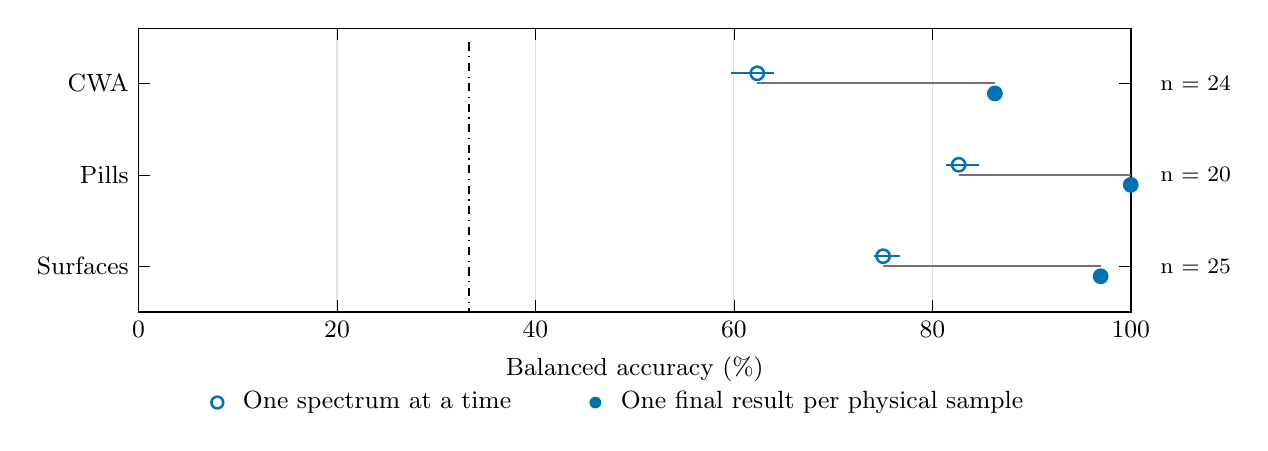
\begin{tikzpicture}
\begin{axis}[briefaxis,width=12.6cm,height=3.6cm,scale only axis,
xmin=0,xmax=100,ymin=-0.6,ymax=2.5,y dir=reverse,
xtick={0,20,40,60,80,100},xmajorgrids=true,
ytick={0,1,2},yticklabels={{CWA},{Pills},{Surfaces}},
xlabel={Balanced accuracy (\%)},clip=false]
\draw[black,dash dot,line width=0.7pt] (axis cs:33.333,-0.45) -- (axis cs:33.333,2.5);
\draw[black!55,line width=0.8pt] (axis cs:62.356760688,0) -- (axis cs:86.309523810,0);
\draw[black!55,line width=0.8pt] (axis cs:82.661401725,1) -- (axis cs:100.000000000,1);
\draw[black!55,line width=0.8pt] (axis cs:75.043180896,2) -- (axis cs:96.969696970,2);
\draw[briefblue,line width=0.6pt] (axis cs:59.711616713,-0.11) -- (axis cs:64.076325039,-0.11);
\addplot[only marks,mark=o,mark size=2.4pt,draw=briefblue,fill=white,line width=0.9pt] coordinates {(62.356760688,-0.11)};
\draw[briefblue,line width=0.6pt] (axis cs:81.386347642,0.89) -- (axis cs:84.707886986,0.89);
\addplot[only marks,mark=o,mark size=2.4pt,draw=briefblue,fill=white,line width=0.9pt] coordinates {(82.661401725,0.89)};
\draw[briefblue,line width=0.6pt] (axis cs:74.083927433,1.89) -- (axis cs:76.783168145,1.89);
\addplot[only marks,mark=o,mark size=2.4pt,draw=briefblue,fill=white,line width=0.9pt] coordinates {(75.043180896,1.89)};
\draw[briefblue,line width=0.6pt] (axis cs:86.309523810,0.11) -- (axis cs:86.309523810,0.11);
\addplot[only marks,mark=*,mark size=2.4pt,draw=briefblue,fill=briefblue,line width=0.9pt] coordinates {(86.309523810,0.11)};
\draw[briefblue,line width=0.6pt] (axis cs:100.000000000,1.11) -- (axis cs:100.000000000,1.11);
\addplot[only marks,mark=*,mark size=2.4pt,draw=briefblue,fill=briefblue,line width=0.9pt] coordinates {(100.000000000,1.11)};
\draw[briefblue,line width=0.6pt] (axis cs:96.969696970,2.11) -- (axis cs:96.969696970,2.11);
\addplot[only marks,mark=*,mark size=2.4pt,draw=briefblue,fill=briefblue,line width=0.9pt] coordinates {(96.969696970,2.11)};
\node[anchor=west,text=black,font=\fontsize{8}{10}\selectfont] at (axis cs:102,0) {n = 24};
\node[anchor=west,text=black,font=\fontsize{8}{10}\selectfont] at (axis cs:102,1) {n = 20};
\node[anchor=west,text=black,font=\fontsize{8}{10}\selectfont] at (axis cs:102,2) {n = 25};
\end{axis}
\draw[briefblue,line width=0.9pt,fill=white] (1, -1.15) circle[radius=0.075];
\node[anchor=west,text=black,font=\fontsize{9}{11}\selectfont] at (1.2,-1.15) {One spectrum at a time};
\fill[briefblue] (5.8,-1.15) circle[radius=0.075];
\node[anchor=west,text=black,font=\fontsize{9}{11}\selectfont] at (6,-1.15) {One final result per physical sample};
\end{tikzpicture}